\RequirePackage{fix-cm}
\documentclass[12pt,a4paper]{book}

% useful packages
\usepackage{microtype}
\usepackage[T1]{fontenc}
\usepackage[utf8]{inputenc}
\usepackage[italian]{babel}

\usepackage[eng,exjobb]{KTHEEtitlepage}

\usepackage{amssymb}
\usepackage{caption}
\usepackage{subcaption}
\usepackage{graphicx,xcolor,textpos}
\usepackage{helvet}
\usepackage{lipsum}
\usepackage{blindtext}
\usepackage{amsmath}
\usepackage{mathtools}
\usepackage{multicol}
\usepackage[super,comma]{natbib}
\usepackage{emptypage}
\usepackage{xcolor}
\usepackage{listings}
\usepackage{xparse}
\usepackage{braket}
\usepackage{verbatim}
\usepackage[font=footnotesize,labelfont=bf]{caption}
\usepackage{listings}

\usepackage{xcolor}
 
\definecolor{codegreen}{rgb}{0,0.6,0}
\definecolor{codegray}{rgb}{0.5,0.5,0.5}
\definecolor{codepurple}{rgb}{0.58,0,0.82}
\definecolor{backcolour}{rgb}{0.95,0.95,0.92}
 
\lstdefinestyle{mystyle}{
    backgroundcolor=\color{backcolour},   
    commentstyle=\color{codegreen},
    keywordstyle=\color{magenta},
    numberstyle=\tiny\color{codegray},
    stringstyle=\color{codepurple},
    basicstyle=\ttfamily\footnotesize,
    breakatwhitespace=false,         
    breaklines=true,                 
 %   captionpos=b,                    
    keepspaces=true,                 
    numbers=left,                    
    numbersep=5pt,                  
    showspaces=false,                
    showstringspaces=false,
    showtabs=false,                  
    tabsize=2
}
 
\lstset{style=mystyle}

\NewDocumentCommand{\codeword}{v}{%
\texttt{\textcolor{blue}{#1}}%
}

% pagina-instellingen
\topmargin -10mm
\textwidth 160truemm
\textheight 240truemm
\oddsidemargin 0mm
\evensidemargin 0mm

\pagestyle{plain}

% instellingen voor hoofdstuknummering en inhoudstafel
\setcounter{secnumdepth}{2} % nummering tot welk subniveau?
\setcounter{tocdepth}{2}

\begin{document}
% FRONT MATTER
\frontmatter
%\thispagestyle{empty}
\newcommand{\form}[1]{\scalebox{1.087}{\boldmath{#1}}}
\sffamily
%
\begin{textblock}{191}(-24,-11)
\colorbox{green}{\hspace{123mm}\ \parbox[c][18truemm]{68mm}{\textcolor{white}{Università degli Studi di Milano}}}
\end{textblock}
%
%\begin{textblock}{70}(-18,-19)
%\textblockcolour{}
%\includegraphics*[height=19.8truemm]{Figuren/LogoKULeuven}
%\end{textblock}
%
\begin{textblock}{160}(-6,63)
\textblockcolour{}
\vspace{-\parskip}
\flushleft
\fontsize{40}{42}\selectfont \textcolor{bluetitle}{Algoritmo per il calcolo del prezzo di derivati finanziari attraverso metodi Monte Carlo in architettura CUDA/C++}\\[1.5mm]
%\fontsize{20}{22}\selectfont Ondertitel \form{$S=\pi r^2$\textsl{(facultatief)}}
\end{textblock}
%
%\begin{textblock}{79}(50,103)
%\textblockcolour{}
%\vspace{-\parskip}
%\flushleft
%\fbox{\parbox{79mm}{De achtergrond kan wit blijven of je kan een afbeelding invoegen (maximum hoogte 10 cm, breedtevariabel, denk aan auteursrechten\ldots). GEEN logo's (je kan binnenin de masterproef logo's gebruiken, maar niet op de voor- %of achterpagina). \textit{Verwijder deze tekstkader.}}}
%\end{textblock}
%
\begin{textblock}{160}(8,153)
\textblockcolour{}
\vspace{-\parskip}
\flushright
\fontsize{14}{16}\selectfont \textbf{Riccardo AIOLFI} \\
\fontsize{14}{16}\selectfont \textbf{Alessandro DE GENNARO} \\
\fontsize{14}{16}\selectfont \textbf{Elena SCIBONA} \\
\end{textblock}
%
\begin{textblock}{70}(-6,191)
\textblockcolour{}
\vspace{-\parskip}
\flushleft
%Promotor: Prof. A. Xyz\\[-2pt]
%\textcolor{blueaff}{Affiliatie \textsl{(facultatief)}}\\[5pt]
%Co-promotor: \textsl{(facultatief)}\\[-2pt]
%\textcolor{blueaff}{Affiliatie \textsl{(facultatief)}}\\[5pt]
%Begeleider: \textsl{(facultatief)}\\[-2pt]
%\textcolor{blueaff}{Affiliatie \textsl{(facultatief)}}\\
\end{textblock}
%
\begin{textblock}{160}(8,191)
%\textblockcolour{}
%\vspace{-\parskip}
%\flushright
%Proefschrift ingediend tot het\\[4.5pt]
%behalen van de graad van\\[4.5pt]
%Bachelor of Science in Xxx\\
\end{textblock}
%
\begin{textblock}{160}(8,232)
\textblockcolour{}
\vspace{-\parskip}
\flushright
Anno Accademico 2019-2020
\end{textblock}
%
\begin{textblock}{191}(-24,248)
{\color{blueline}\rule{550pt}{5.5pt}}
\end{textblock}
%
\vfill
 \cleardoublepage 
% COVER PAGE
\ititle{\textsc{Pricing di derivati finanziari tramite tecniche Monte Carlo\\ in architettura CUDA/C++}}
\makeititle
\rmfamily

%\thispagestyle{empty}
\setlength{\parindent}{0cm}
\vspace*{\fill}
De auteur en promotor geven de toelating deze scriptie voor consultatie beschikbaar te stellen en delen ervan te kopi¨eren voor persoonlijk gebruik. Elk ander gebruik valt onder de beperkingen van het auteursrecht, in het bijzonder met betrekking tot de verplichting uitdrukkelijk de bron te vermelden bij het aanhalen van resultaten uit deze scriptie.\par
\vspace{0.4cm}
Leuven, 11 Juni 2019 \par
\vspace{0.5cm}
Promotoren \hfill Auteur \par 
\vspace{1cm}
Professor 1  \\
Professor 2 \hfill Student \\
\setlength{\parindent}{0.5cm}
 \cleardoublepage
\setcounter{page}{0}
\pagenumbering{alph}

%\addcontentsline{toc}{chapter}{Prefazione}
\chapter*{Prefazione}
\lipsum[1] \clearpage{\pagestyle{plain}\cleardoublepage}
%\addcontentsline{toc}{chapter}{Samenvatting}
\chapter*{Samenvatting}
\lipsum[1] \cleardoublepage

\addcontentsline{toc}{chapter}{Sommario}
\tableofcontents \cleardoublepage
% MAIN MATTER
\mainmatter
\setcounter{page}{0}
\pagenumbering{arabic}

\chapter{(A) Introduzione alla libreria e aspetti implementativi}
\section{Econofisica e \textit{option pricing}} \label{sec:introduction_econophysic_option_pricing}
In ambito finanziario si definisce \textit{titolo derivato} un contratto il cui valore dipende da prodotto finanziario più fondamentale, detto \textit{bene sottostante} o semplicemente \textit{sottostante}. Obiettivo di questa relazione è lo studio di un tipo particolare di titolo derivato, ovvero le \textit{opzioni europee}, nella loro forma più elementare definibili come contratti che garantiscono il diritto di compravendita del sottostante in una data futura (detta \textit{data di maturità}) a un prezzo fissato (detto \textit{prezzo di esercizio}). A seconda delle caratteristiche del tipo di opzione prescelto, ciò frutterà al suo acquirente un rendimento $P$ detto \textit{payoff}.

Un primo esempio di contratto derivato analizzato in questa trattazione è il contratto a termine \textit{forward}, con un \textit{payoff} definito da
\begin{equation}
    P_f = S(T),
    \label{eq:forward_payoff}
\end{equation}
dove $T$ è la data di maturità e $S(t)$ il prezzo del sottostante al tempo $t$. Altra tipologia importante di opzioni è quella delle opzioni \textit{plain vanilla}, definite come \textit{call} o \textit{put} a seconda che diano il diritto di comprare o vendere il sottostante. Nel caso delle \textit{plain vanilla call} il \textit{payoff} è dato da
\begin{equation}
    P_{pvc} = \Theta(S(T)-E),
    \label{eq:pvc_payoff}
\end{equation}
mentre nelle \textit{plain vanilla put} è dato da
\begin{equation}
    P_{pvp} = \Theta(E-S(T)),
    \label{eq:pvp_payoff}
\end{equation}
dove $E$ è il prezzo di esercizio e $\Theta(x)$ è la funzione di Heaviside.

Un esempio di opzione più sofisticata, che sarà anche l'oggetto principale di studio della relazione, è costituito dall'opzione di tipo \textit{performance corridor}, il cui \textit{payoff} è dato da
\begin{equation}
    P_{pc} = N\left[ \frac{1}{m} \sum_{i=0}^{m-1}{P_i} - K \right]^+,
    \label{eq:performancecorridor_payoff}
\end{equation}
dove $+$ indica la parte positiva dell'espressione e
\begin{equation}
    P_i = \begin{cases}
    1, & \text{se} \,\,\left| \frac{1}{\sqrt{\Delta t}} \ln{\frac{S(t_{i+1})}{S(t_i)}} \right| < B \sigma;\\
    0, & \text{altrimenti}.
  \end{cases}
    \label{eq:performancecorridor_barrier}
\end{equation}

Questo è un caso di opzione \textit{path-dependent}, in quanto il \textit{payoff} è funzione della percentuale di volte in cui il rendimento logaritmico del sottostante in modulo tra due date di rilevazione rimane confinato all'interno di una barriera la cui altezza è parametrizzata da $B$. In questo contesto la variabile $K$ rappresenta una sorta di <<prezzo di esercizio>> in percentuale, mentre $N$ è il nozionale a cui la percentuale risultante dal calcolo del \textit{payoff} viene applicata.

In virtù dell'\textit{assioma di non arbitraggio}, il quale afferma che non è possibile realizzare un guadagno certo a un rendimento superiore al tasso di interesse privo di rischio, il prezzo equo delle opzioni è stabilito sulla base del \textit{payoff} delle opzioni stesse. Essendo quest'ultimo dipendente dall'andamento del prezzo del sottostante tra la data odierna e la data di maturità, il problema del \textit{pricing} delle opzioni è legato a doppio filo alla necessità di modellizzare l'evoluzione del sottostante nel tempo.

Uno dei modelli più diffusi per questo scopo è quello del \textit{moto browniano geometrico}, basato sull'assunto che il prezzo $S(t)$ del sottostante segua un processo lognormale con tasso d'interesse privo di rischio $r$ e volatilità $\sigma$ fissata
\begin{equation}
    \frac{dS}{S} = r dt + \sigma \sqrt{dt} w,
    \label{eq:lognormal}
\end{equation}
dove $w$ è una variabile casuale estratta da una distribuzione normale di media nulla e varianza unitaria. Dividendo l'intervallo $[0,T]$ in $m$ date di rilevazione $t_i$ di distanza $\Delta t$, si calcola il prezzo $S(t_{i+1})$ in funzione del prezzo attuale $S(t_i)$ secondo la formula
\begin{equation}
    S(t_{i+1}) = S(t_i) \exp{\left[\left(r- \frac{\sigma^2}{2}\right)\Delta t + \sigma \sqrt{\Delta t} w\right]}.
    \label{eq:exactprice}
\end{equation}

Nell'approssimazione di un intervallo $\Delta t$ sufficientemente ridotto\footnote{Per un approfondimento sui limiti di applicabilità di questa approssimazione, consultare la Sezione \ref{sec:limits}.}, l'equazione \eqref{eq:lognormal} può essere risolta con una tecnica semplificata arrivando alla formula alternativa
\begin{equation}
    S(t_{i+1}) \approx S(t_i) \left(1 + r \Delta t + \sigma \sqrt{\Delta t} w\right).
    \label{eq:eulerprice}
\end{equation}

Nel corso della relazione faremo riferimento alla soluzione \eqref{eq:exactprice} come \textit{schema esatto} e alla \eqref{eq:eulerprice} come \textit{schema di Eulero}. Iterando questi schemi sull'intero lasso di tempo d'elezione è possibile effettuare \textit{simulazioni} dell'evoluzione del prezzo del sottostante e conseguentemente stabilire il \textit{payoff} medio di un'opzione alla data di maturità.

Ciò non è tuttavia sufficiente a determinare il prezzo equo dell'opzione, poiché il valore di un determinato capitale in data odierna $T_0$ non corrisponde al valore del medesimo capitale in una data futura $T>T_0$; ciò avviene perché la definizione stessa di tasso di interesse \textit{privo di rischio} implica che il denaro nel tempo è in grado di generare con probabilità certa ulteriore denaro. Per tale ragione è necessario \textit{attualizzare} il \textit{payoff} attraverso la formula
\begin{equation}
    P_0 = P_T e^{-rT}.
    \label{actualization}
\end{equation}


\section{Panoramica del codice} \label{sec:code_generics}
Le caratteristiche del problema dell'\textit{option pricing} lo rendono particolarmente adatto a essere affrontato con una metodologia di tipo \textit{single instruction, multiple data} (SIMD), un'architettura in cui un insieme di elementi processori eseguono il medesimo algoritmo su flussi di dati differenti; un codice progettato secondo questa filosofia sarà infatti in grado di eseguire un elevato numero di simulazioni del prezzo del sottostante in parallelo, ottimizzando i tempi di esecuzione.

La piattaforma di sviluppo CUDA progettata dalla Nvidia Corporation si presta in modo particolare a questo tipo di architettura in quanto le GPU su cui il codice viene eseguito sono caratterizzate da un elevato numero di \textit{core} in grado di eseguire operazioni elementari. La libreria oggetto di questa relazione è stata quindi da noi sviluppata in linguaggio CUDA/C++ per trarre vantaggio di tali peculiarità; per una discussione più approfondita circa i vantaggi di questo approccio rispetto al più semplice CUDA/C, riferirsi al Capitolo \ref{cap:cudacpp}.

In Figura (FIGURA) è riportato un diagramma riassuntivo del funzionamento dell'eseguibile primario della libreria, orientato all'\textit{option pricing}. Il listato integrale del codice appositamente commentato è riportato in Appendice \ref{app:allcode}; a seguire ne saranno illustrati i punti principali.

Al primo livello di complessità, classi, strutture e funzioni di supporto della libreria da noi progettata sono suddivise in tre macrocategorie:

\begin{itemize}
    \item \textbf{strutture di \textit{input}}: strutture elementari per la memorizzazione dei dati riguardanti le opzioni (\codeword{Input_option_data}), il mercato (\codeword{Input_market_data}), la GPU (\codeword{Input_GPU_data}) e la simulazione Monte Carlo (\codeword{Input_MC_data});
    \item \textbf{struttura di \textit{output}}: struttura singola (\codeword{Output_MC_data}) che raccoglie i risultati delle simulazioni Monte Carlo;
    \item \textbf{librerie principali}: classi C++ che gestiscono e manipolano i dati nelle simulazioni, discusse di seguito.
\end{itemize}

La prima libreria principale per ordine logico è la classe astratta \codeword{RNG} che gestisce la generazione di numeri pseudocasuali. Nel codice sono implementate due tipologie di generatori concreti: un generatore Tausworthe puro basato su un registro a scorrimento a retroazione lineare (\codeword{RNG_Tausworthe}) e un generatore combinato basato su tre generatori Tausworthe e un generatore lineare congruenziale (\codeword{RNG_CombinedGenerator}).

A partire dai numeri generati da un puntatore \codeword{RNG*}, la classe \codeword{Path} gestisce i singoli passi del processo lognormale esatto \eqref{eq:exactprice} e della versione approssimata di Eulero \eqref{eq:eulerprice}, calcolando il \textit{payoff} $P_i$ delle opzioni. Questi ultimi sono processati dalla classe \codeword{Statistics}, che ne calcola la media $\braket{P_i}$ e l'errore
\begin{equation}
    \epsilon_\text{MC} = \sqrt{\frac{\frac{1}{N}\sum_i{P_i^2} - \braket{P_i}^2}{N}}
    \label{eq:mcerror}
\end{equation}

Infine la classe \codeword{Data_stream_manager} gestisce l'interazione dell'utente con il flusso di dati in entrata e in uscita, interpretando i dati indicati nel file \verb|input.dat|, scrivendo i risultati di \textit{output} in un oggetto \codeword{Output_MC_data} e stampando a schermo le informazioni sulle simulazioni effettuate.

L'interazione tra le varie componenti del codice è organizzata dal metodo  \codeword{OptionPricingEvaluator(...)}, programmato nelle sue varianti \codeword{__global__}, \codeword{__host__} e \codeword{__device__ __host__} secondo il paradigma \textit{host-device} approfondito in Sezione \ref{sec:cpugpu}. La funzione principale \codeword{main()}, secondo i desideri dell'utente, esegue tale algoritmo su CPU o GPU invocando due funzioni ausiliarie \codeword{CPUOptionPricingMonteCarloAlgorithm(...)} e \codeword{CPUOptionPricingMonteCarloAlgorithm(...)}.

\begin{table}[t]
\small
\centering
\begin{tabular}{|l||l|l|}
\hline
\textbf{GPU} & \textit{Tesla P100-PCIE-12GB} & \textit{Tesla C2075} \\
\hline \hline
\textbf{CUDA Driver version} & 10.1 & 9.1 \\ \hline
\textbf{CUDA Runtime version} & 10.1 & 8.0 \\ \hline
\textbf{CUDA Capability version} & 6.0 & 2.0 \\ \hline
\textbf{Global memory} & 12 GB &  5 GB \\ \hline
\textbf{Maximum clock rate} & 1.33 GHz & 1.15 GHz \\ \hline
\textbf{Multiprocessors} & 56 & 14 \\ \hline
\textbf{CUDA Cores} & 3584 & 448 \\ \hline
\textbf{Constant memory} & 65 kB & 65 kB \\ \hline
\textbf{Shared memory per block} & 49 kB & 49 kB \\
\hline
\end{tabular}
\caption{Specifiche tecniche delle due schede grafiche in nostra dotazione per le simulazioni.}
\label{tab:hardware}
\end{table}

\section{Specifiche hardware} \label{sec:hardware}
La maggior parte delle simulazioni da cui sono stati ottenuti i risultati illustrati nella presente relazione è stata effettuata su una scheda grafica di modello \verb|Tesla P100-PCIE-12GB|. Occasionalmente, e in modo significativo negli studi sul tempo di esecuzione in Sezione \ref{sec:comptime}, abbiamo fatto uso di una meno performante \verb|Tesla C2075|. In Tabella \ref{tab:hardware} sono riportate le specifiche hardware delle due GPU.
\chapter{(B) Risultati numerici relativi al \textit{pricing} Monte Carlo}
Menzionare i dati <<standard>> delle simulazioni.
\section{(B-1) Controlli di affidabilità dei risultati}
\subsection{(B-1-i) Corrispondenza tra risultati in CPU e GPU} \label{sec:cpugpu}
\lipsum[1-3]
\subsection{(B-1-ii) Corrispondenza tra risultati e valori calcolati analiticamente}
\lipsum[1-3]


\section{(B-2) Controlli di autocorrelazione nella generazione di numeri casuali}

Come brevemente illustrato in Sezione \ref{sec:code_generics}, il nucleo dell'algoritmo di simulazione del prezzo del sottostante è costituito dal generatore combinato di numeri pseudocasuali che produce le variabili gaussiane di media nulla e varianza unitaria necessarie per applicare lo schema esatto e lo schema di Eulero. Ciascuno di tali numeri $z_i$ è ottenuto tramite il metodo della trasformata di Box-Muller
\begin{equation}
    z_i = \sqrt{-2 \ln{u_i}} \cos{\left(2\pi v_i\right)}
    \label{eq:BoxMuller}
\end{equation}
a partire da una precedente coppia di numeri pseudocasuali $u_i, v_i$ estratti uniformemente nell'intervallo $[0,1]$. Ogni oggetto della classe \codeword{RNG_Combined} richiede quattro \textit{seed} per essere inizializzato; poiché questi \textit{seed} devono differire per ciascun \textit{thread} in quanto ogni \textit{thread} deve produrre un flusso indipendente di numeri pseudocasuali, abbiamo scelto di generare tali valori iniziali con l'ausilio di un generatore di supporto \codeword{RNG_Tausworthe}, generatore Tausworthe puro che viene inizializzato con un singolo \textit{seed}. Questo seme può essere scelto casualmente utilizzando la funzione \codeword{time()} della libreria C \codeword{time.h} oppure può essere fissato per garantire riproducibilità dei risultati.

In virtù della complessità del nostro apparato non-standard di generazione di numeri casuali e della sua centralità nel progetto di \textit{option pricing}, abbiamo svolto controlli approfonditi per verificare che le proprietà delle distribuzioni di estrazione corrispondessero alle attese e che non sorgessero distorsioni di autocorrelazione all'interno di un \textit{thread} (\textit{intra-stream}) e tra i flussi prodotti da \textit{thread} differenti (\textit{inter-stream}). A titolo di esempio abbiamo esaminato $512000$ numeri generati equamente da 512 \textit{thread} diversi, ciascuno istanziato con una propria quaterna di \textit{seed} pseudocasuali.

\begin{figure}[t]
\centering
\begin{subfigure}{.5\textwidth}
  \centering
  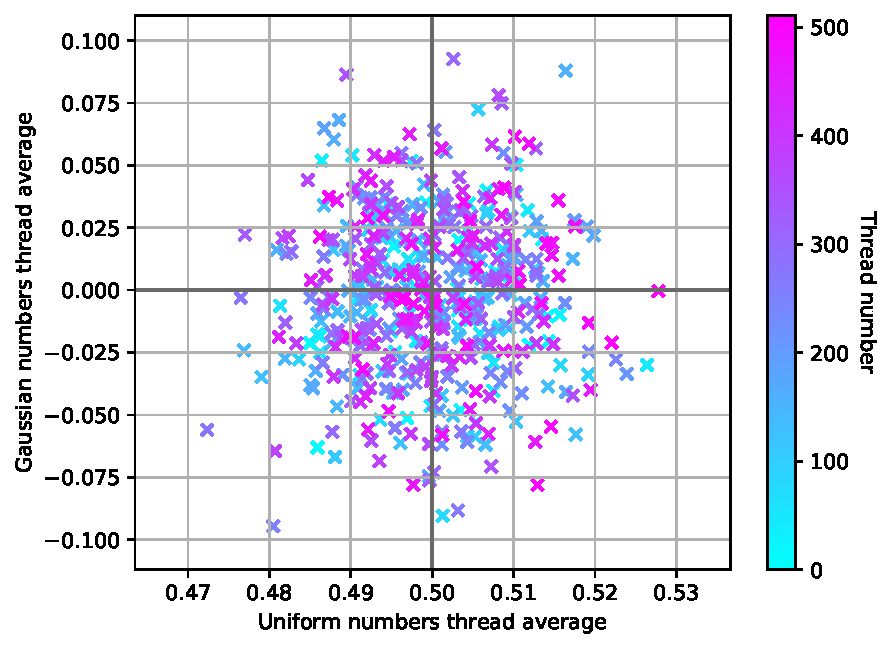
\includegraphics[scale=0.5]{graphs/CorrelationTests_UniAvgVsGaussAvg.pdf}
  \caption{}
  \label{fig:unigauss_avg}
\end{subfigure}%
\begin{subfigure}{.5\textwidth}
  \centering
  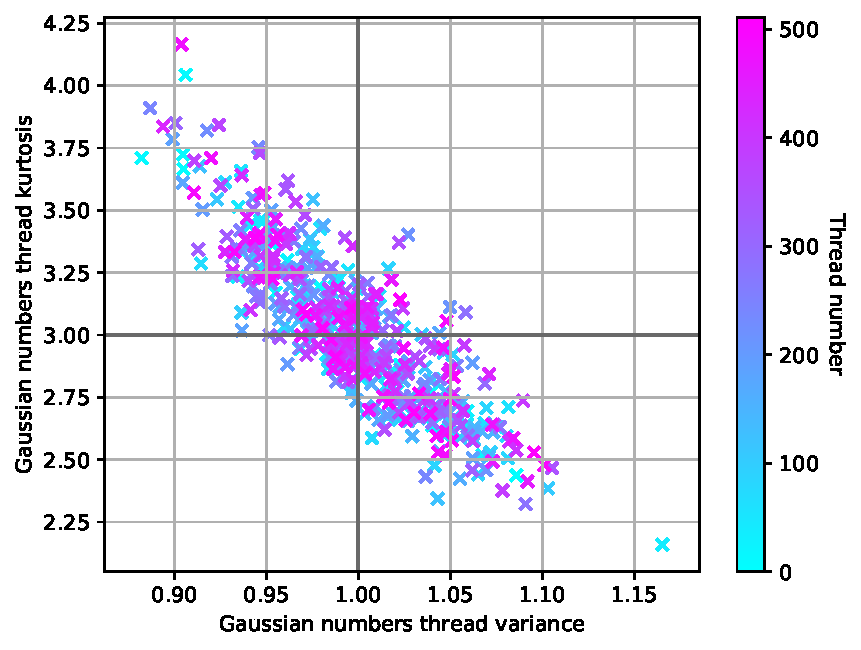
\includegraphics[scale=0.5]{graphs/CorrelationTests_KurtosisVsVariance.pdf}
  \caption{}
  \label{fig:variance_kurt}
\end{subfigure}
\caption{Dispersione di valori medi dei flussi di numeri pseudcasuali generati da ciascun \textit{thread} della GPU, il cui numero da 0 a 511 è indicato in scala cromatica da \textit{ciano} a \textit{magenta}. \textit{(a)} Dispersione delle medie dei numeri casuali generati nell'intervallo $[0,1]$ (ascissa) e dei numeri estratti da una distribuzione normale di media nulla e varianza unitaria (ordinata); \textit{(b)} dispersione di varianza e curtosi dei numeri estratti dalla medesima distribuzione normale di cui sopra. Le rette in \textit{grigio} evidenziano i valori teorici attesi per le quantità rappresentate: $\frac{1}{2}$ per la media di numeri uniformi, $0$, $1$ e $3$ per media, varianza e curtosi della distribuzione gaussiana.} 
\end{figure}

Per cominciare, in Figura \ref{fig:unigauss_avg} sono riportate le medie in ciascun \textit{thread} dei valori assunti dai numeri estratti uniformemente (in ascissa) e dai numeri estratti gaussianamente (in ordinata); come evidenziato dalla scala cromatica che indica il numero di \textit{thread}, la dispersione delle medie rispetto ai valori attesi indicati dalle rette in grigio non presenta asimmetrie significative. Un discorso analogo può essere fatto per la Figura \ref{fig:variance_kurt}, che riporta in ascissa la varianza
\begin{equation}
    \sigma^2 = \braket{{\left(r-\braket{r}\right)}^2}
    \label{eq:variance}
\end{equation}
e in ordinata la curtosi
\begin{equation}
    \text{Kurt}[r] = \frac{\braket{{\left(r-\braket{r}\right)}^4}}{\sigma^4}
    \label{eq:kurtosis}
\end{equation}
dei numeri generati gaussianamente, fatto salvo il \textit{caveat} che le due variabili sono evidentemente anticorrelate per la definizione di curtosi.

\begin{figure}[t]
\centering
\begin{subfigure}{.5\textwidth}
  \centering
  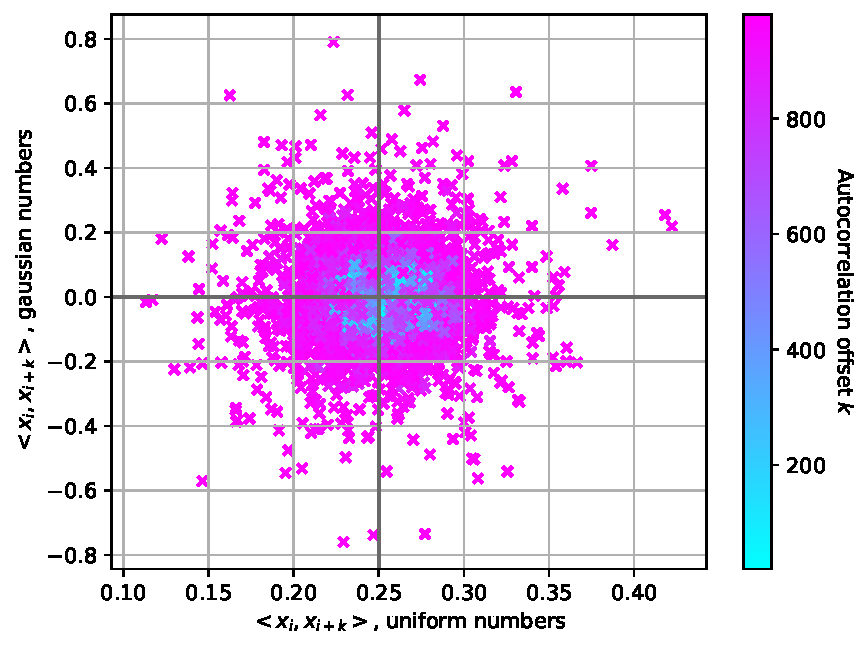
\includegraphics[scale=0.5]{graphs/CorrelationTests_IntraStreamCorrelations.pdf}
  \caption{}
  \label{fig:intra_corr}
\end{subfigure}%
\begin{subfigure}{.5\textwidth}
  \centering
  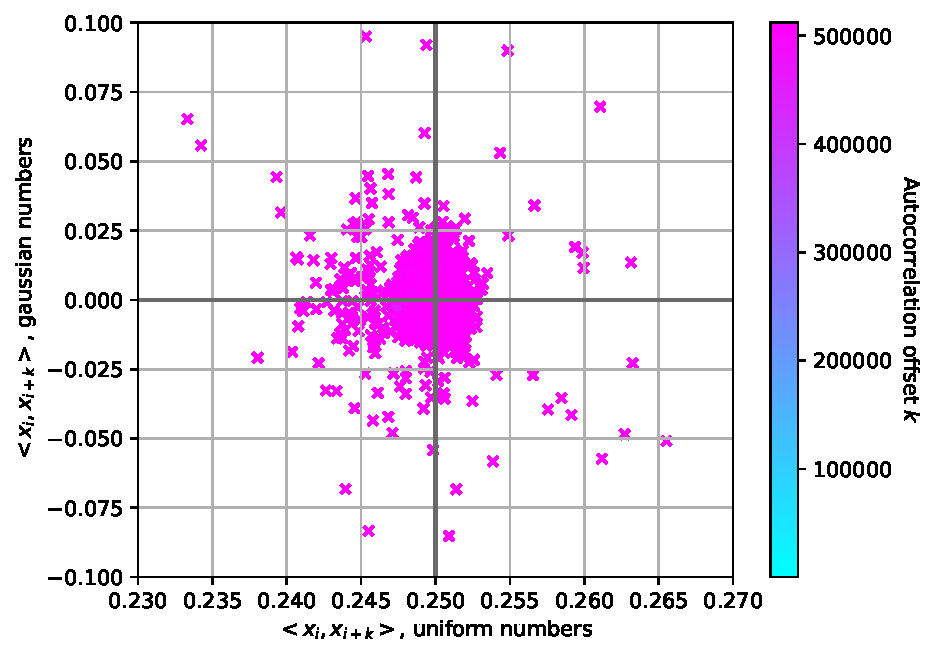
\includegraphics[scale=0.5]{graphs/CorrelationTests_InterStreamCorrelations.pdf}
  \caption{}
  \label{fig:inter_corr}
\end{subfigure}
\caption{Confronto tra autocorrelazioni $\braket{x_i x_{i+k}}$ nei casi di \textit{(a)} controllo \textit{intra-stream} sui flussi prodotti dai 512 \textit{thread}, e \textit{(b)} controllo \textit{inter-stream} effettuato su un singolo \textit{superstream} definito come in EQUAZIONE. In ascissa è riportata l'autocorrelazione nei flussi di numeri estratti uniformemente nell'intervallo $[0,1]$, in ordinata l'autocorrelazione dei numeri estratti secondo la distribuzione normale di media nulla e varianza unitaria; in scala cromatica da \textit{ciano} a \textit{magenta} è riportato il valore di $k$, mentre le rette in \textit{grigio} riportano i valori attesi ($\frac{1}{4}$ per la correlazione tra i numeri uniformi, $0$ per quella tra i numeri gaussiani).}
\end{figure}

Più spinoso è il caso della \textit{correlazione} $\braket{x_i x_{i+k}}$, dove $k$ è detto \textit{offset}. In Figura \ref{fig:intra_corr} è riportata la correlazione \textit{intra-stream} per i numeri distribuiti uniformemente (ascissa) e gaussianamente (ordinata). La scala cromatica questa volta indica l'\textit{offset} $k$, evidenziando come per $k$ elevati la dispersione dei risultati rispetto ai valori attesi (in grigio) sia fisiologicamente superiore in quanto sono disponibili meno numeri su cui effettuare la media. Ciononostante la distribuzione rimane visibilmente simmetrica e, pur non essendo evidenziati i risultati dei singoli \textit{thread}, studi in questa direzione non hanno evidenziato parzialità.

La Figura \ref{fig:inter_corr} riporta risultati secondo il medesimo schema della precedente applicati a un <<\textit{super-stream}>> ottenuto combinando tutti i 512 \textit{thread} secondo la formula
\begin{equation}
    w_{k=iN+j} = r_j^i,
    \label{eq:superstream}
\end{equation}
dove $j=1,...,512$ è l'indice di \textit{thread} e $i=1,...,1000$ è l'indice di numero generato. Se i numeri gaussiani preservano una distribuzione simmetrica intorno alla correlazione attesa, in quelli gaussiani spicca una polarizzazione a favore di valori leggermente inferiori a $\frac{1}{4}$.

\begin{figure}[t]
\centering
\begin{subfigure}{.5\textwidth}
  \centering
  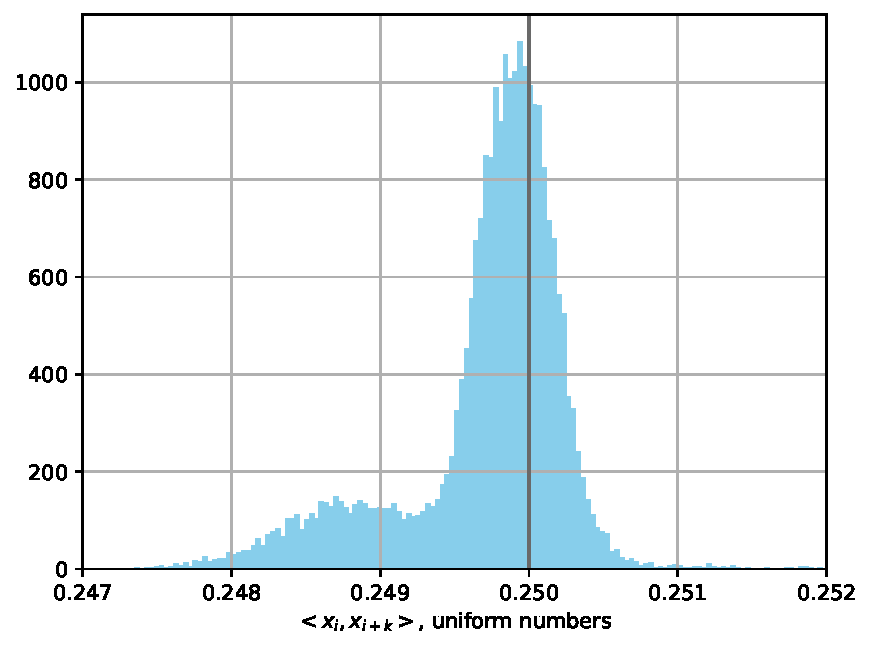
\includegraphics[scale=0.5]{graphs/CorrelationTests_UniformInterStreamAutocorrelationHistogram.pdf}
  \caption{}
  \label{fig:inter_uni_autocorr_histo}
\end{subfigure}%
\begin{subfigure}{.5\textwidth}
  \centering
  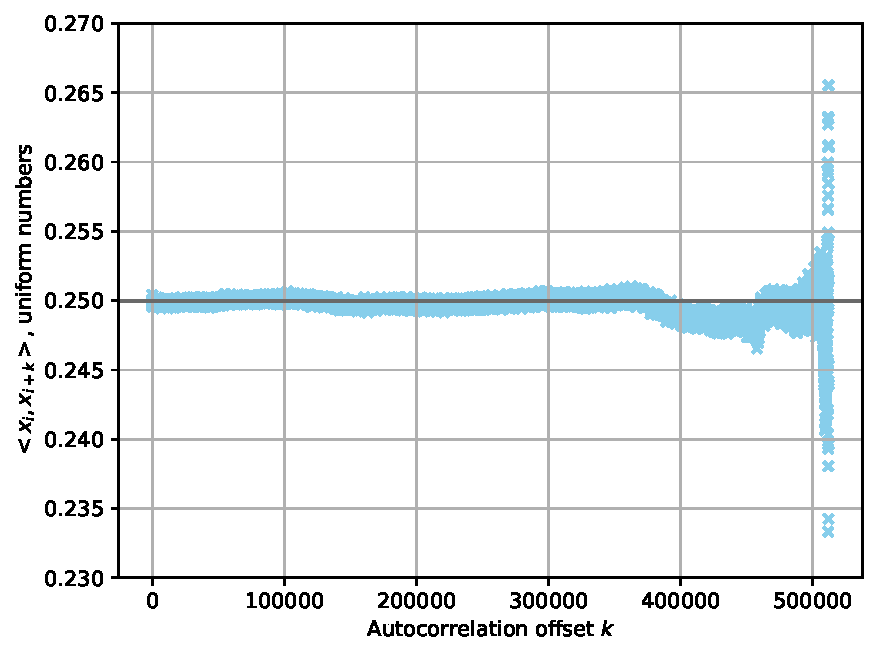
\includegraphics[scale=0.5]{graphs/CorrelationTests_UniformInterStreamAutocorrelationVsOffset.pdf}
  \caption{}
  \label{fig:inter_uni_autocorr_offset}
\end{subfigure}
\caption{\textit{(a)} Istogramma delle autocorrelazioni $\braket{x_i x_{i+k}}$ \textit{inter-stream} del flusso di numeri pseudocasuali estratti uniformemente nell'intervallo $[0,1]$; \textit{(b)} andamento delle correlazioni in funzione dell'\textit{offset} $k$.}
\end{figure}

Per indagare più a fondo questa distorsione abbiamo riportato in Figura \ref{fig:inter_uni_autocorr_histo} un istogramma delle correlazioni \textit{inter-stream} dei numeri uniformi e in Figura \ref{fig:inter_uni_autocorr_offset} il suo andamento in funzione di $k$. Da questi grafici è evidente come il picco secondario appaia per \textit{offset} particolarmente alti; ciononostante, anche l'andamento prima dell'anomalia presenta una forma vagamente oscillatoria, evidenziando come il flusso di numeri pseudocasuali non soddisfi pienamente la richiesta di autoindipendenza.

\begin{figure}[t]
\centering
\begin{subfigure}{.5\textwidth}
  \centering
  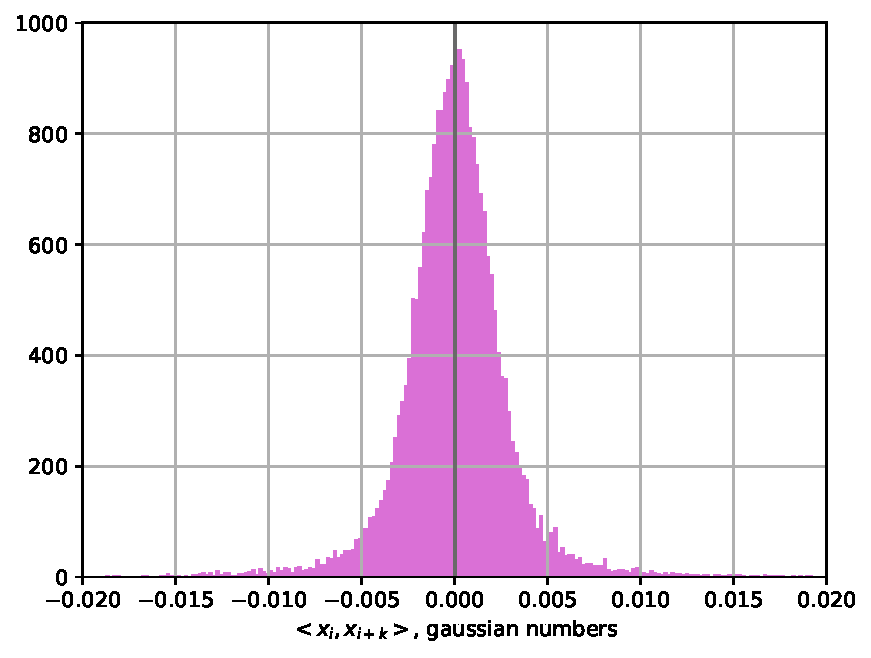
\includegraphics[scale=0.5]{graphs/CorrelationTests_GaussInterStreamAutocorrelationHistogram.pdf}
  \caption{}
  \label{fig:inter_gauss_autocorr_histo}
\end{subfigure}%
\begin{subfigure}{.5\textwidth}
  \centering
  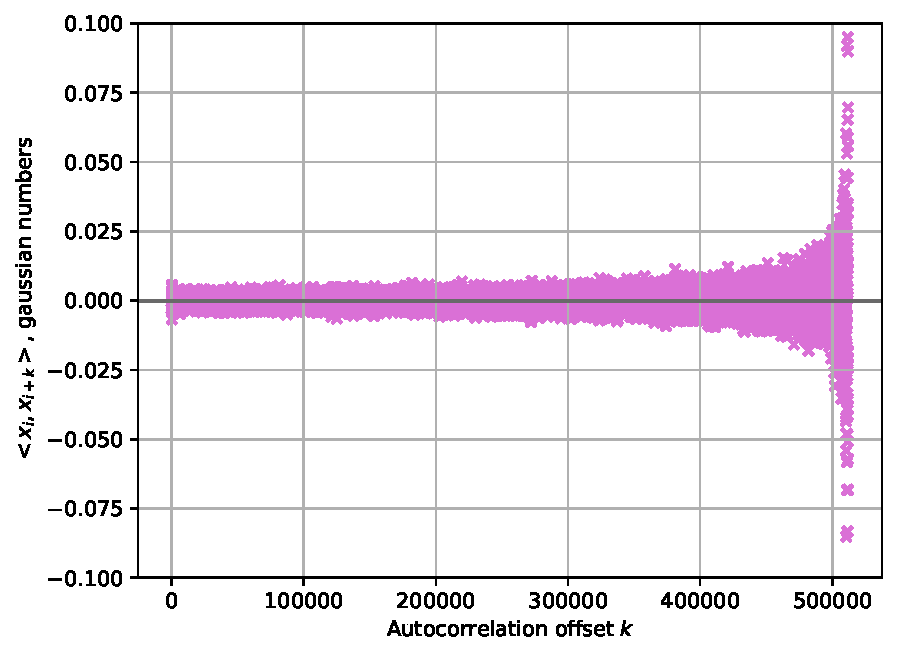
\includegraphics[scale=0.5]{graphs/CorrelationTests_GaussInterStreamAutocorrelationVsOffset.pdf}
  \caption{}
  \label{fig:inter_gauss_autocorr_offset}
\end{subfigure}
\caption{\textit{(a)} Istogramma delle autocorrelazioni $\braket{x_i x_{i+k}}$ \textit{inter-stream} del flusso di numeri pseudocasuali estratti uniformemente secondo una distribuzione normale di media nulla e varianza unitaria; \textit{(b)} andamento delle correlazioni in funzione dell'\textit{offset} $k$.}
\end{figure}

Ciononostante, le analoghe Figure \ref{fig:inter_gauss_autocorr_histo} e \ref{fig:inter_gauss_autocorr_offset} evidenziano come, pur essendo i numeri gaussiani generati a partire da quelli uniformi, in essi sia essenzialmente assente ogni spettro di autocorrelazione. Poiché le variabili gaussiane sono quelle di reale interesse, i controlli effettuati avvalorano l'indipendenza e l'affidabilità delle nostre simulazioni.

\section{(B-3) \textit{Pricing} dell'opzione \textit{performance corridor}}
\subsection{(B-3-a) Dipendenza dalle date di rilevamento e dal numero di simulazioni}

\begin{figure}[t]
    \centering
    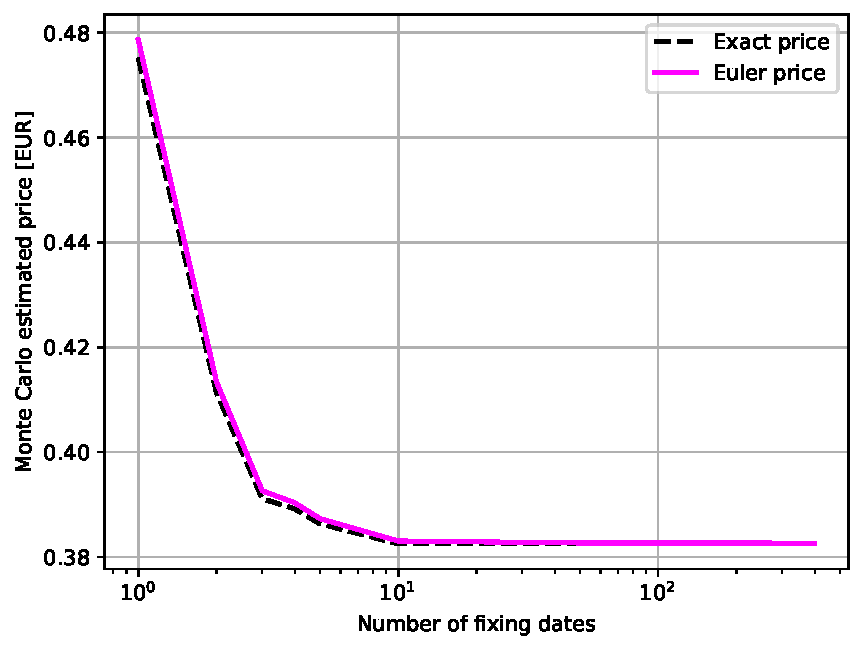
\includegraphics[scale=0.5]{graphs/OptionPriceVsM_PriceVsM_N100mln.pdf}
    \caption{Confronto dell'andamento del prezzo dell'opzione \textit{performance corridor} in funzione del numero di date di rilevamento calcolato secondo lo schema di Eulero (\textit{magenta}) e secondo lo schema esatto (\textit{nero}, \textit{tratteggiato}).}
    \label{fig:exactvseuler_M}
\end{figure}

\begin{figure}[t]
    \centering
    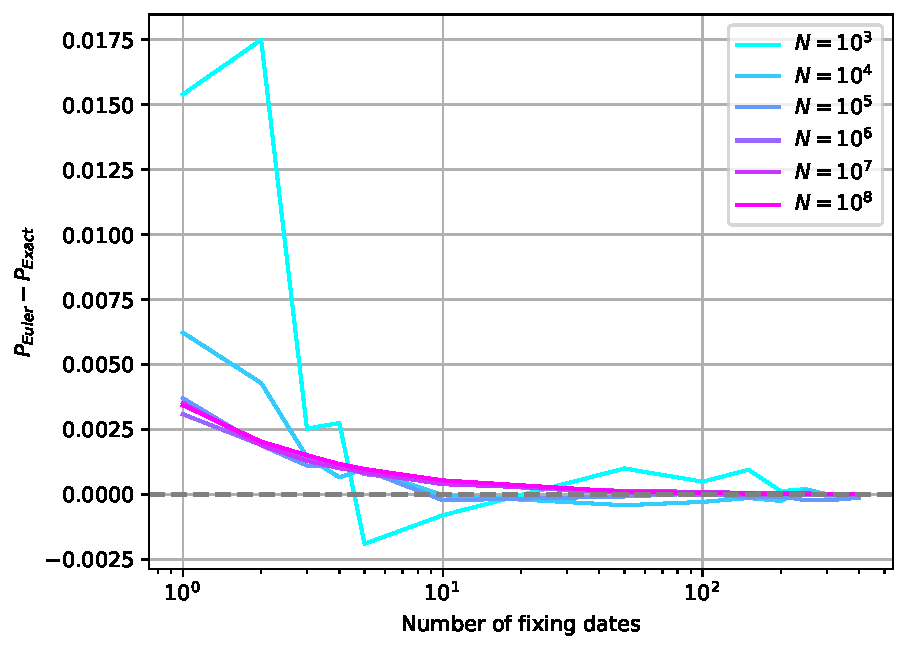
\includegraphics[scale=0.5]{graphs/OptionPriceVsM_DiscrepancyVsM_WithDifferentNs.pdf}
    \caption{Differenza tra i prezzi dell'opzione \textit{performance corridor} calcolati secondo lo schema di Eulero e secondo lo schema esatto in funzione del numero di date di rilevamento; da \textit{ciano} a \textit{magenta} curve con numero crescente di simulazioni da ${10}^3$ a ${10}^8$, in \textit{grigio tratteggiato} il valore asintotico di discrepanza nulla.}
    \label{fig:ex_eul_discrep_M}
\end{figure}

\lipsum[1-3]

\subsection{(B-3-b) Dipendenza dal valore di $B$}

\begin{figure}[t]
    \centering
    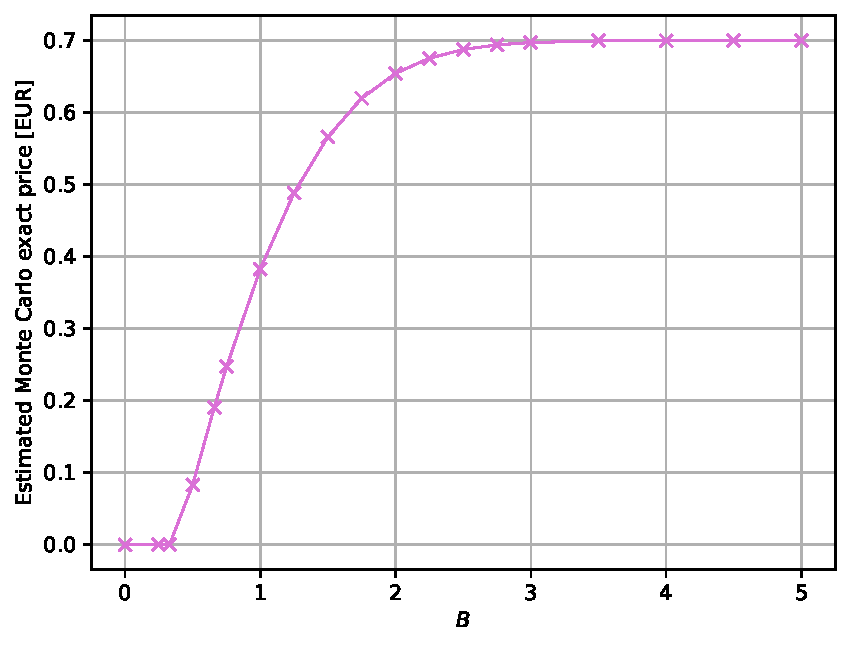
\includegraphics[scale=0.5]{graphs/OptionPriceVsB_PriceVsB_N200mln.pdf}
    \caption{Andamento del prezzo dell'opzione \textit{performance corridor} stimato secondo lo schema esatto in funzione del parametro $B$ che determina l'altezza della barriera.}
    \label{fig:price_vs_b}
\end{figure}

\lipsum[1-3]


\section{(B-4) Studi sull'errore Monte Carlo}
\subsection{(B-4-a) Dipendenza dalle date di rilevamento e dal numero di simulazioni}

\begin{figure}[t]
\centering
\begin{subfigure}{.5\textwidth}
  \centering
  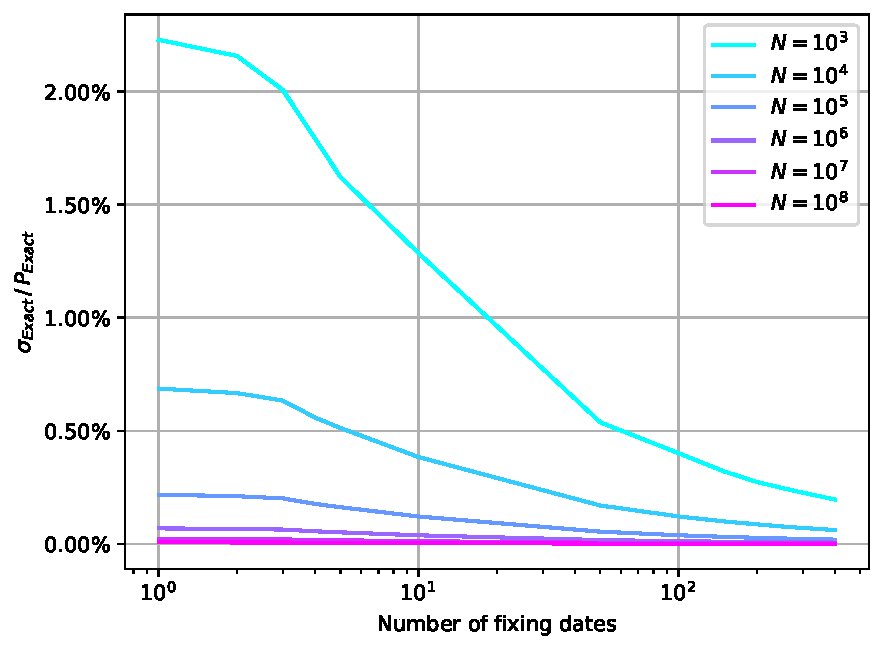
\includegraphics[scale=0.5]{graphs/OptionPriceVsM_ExactErrorVsM_WithDifferentNs.pdf}
  \caption{}
  \label{fig:exact_error_M}
\end{subfigure}%
\begin{subfigure}{.5\textwidth}
  \centering
  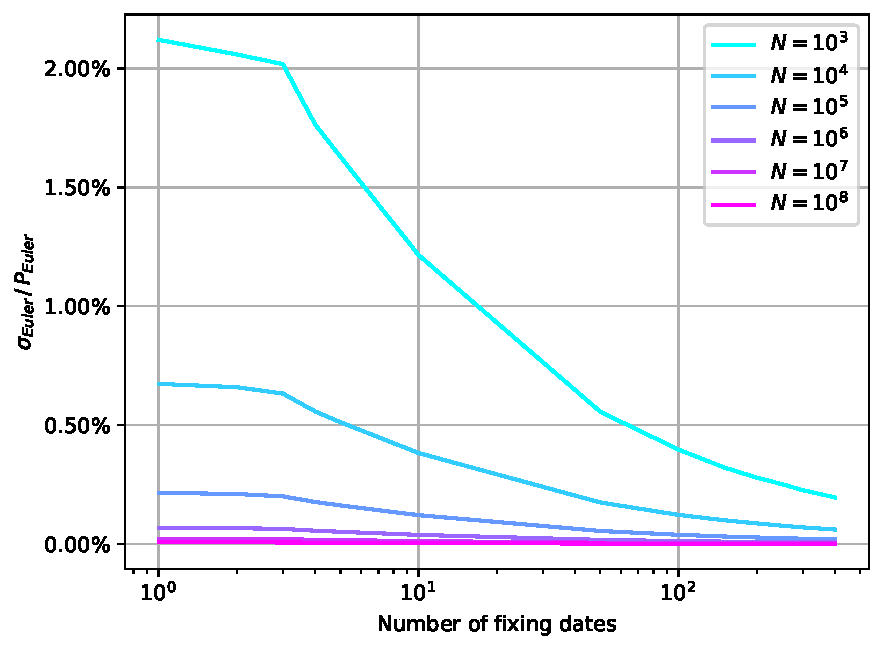
\includegraphics[scale=0.5]{graphs/OptionPriceVsM_EulerErrorVsM_WithDifferentNs.pdf}
  \caption{}
  \label{fig:euler_error_M}
\end{subfigure}
\caption{Andamento dell'errore relativo Monte Carlo in funzione del numero di date di rilevamento rispetto al prezzo calcolato \textit{(a)} secondo lo schema esatto e \textit{(b)} secondo lo schema di Eulero; curve di colore da \textit{ciano} a \textit{magenta} corrispondono a un numero crescente di simulazioni da ${10}^3$ a ${10}^8$.}
\end{figure}

\lipsum[1-3]

\subsection{(B-4-b) Dipendenza dal valore di $B$}

\begin{figure}[t]
    \centering
    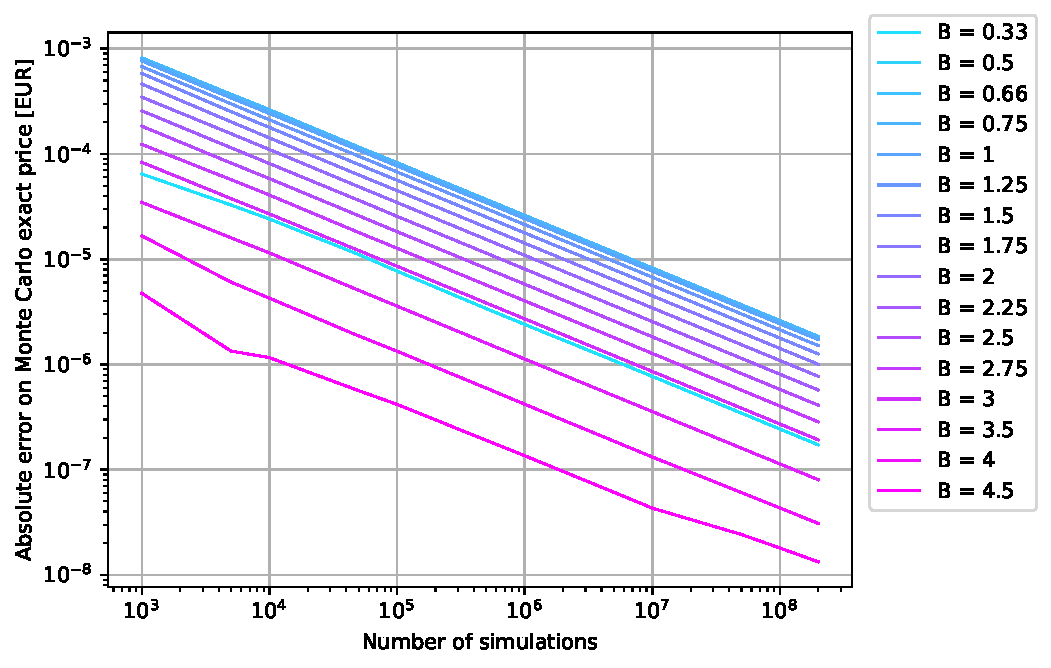
\includegraphics[scale=0.5]{graphs/OptionPriceVsB_ExactErrorVsN_WithAllBs.pdf}
    \caption{Errore assoluto Monte Carlo rispetto al prezzo calcolato secondo lo schema esatto in funzione del numero di simulazioni effettuate; curve di colore da \textit{ciano} a \textit{magenta} corrispondono a valori crescenti del parametro $B$.}
    \label{fig:error_vs_B}
\end{figure}

\begin{figure}[t]
    \centering
    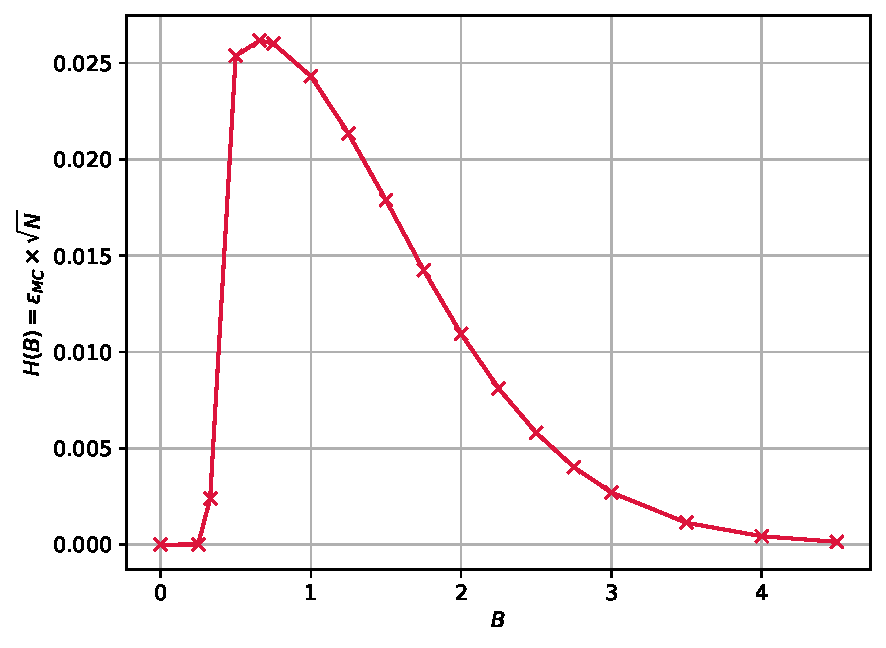
\includegraphics[scale=0.5]{graphs/OptionPriceVsB_HBVsB.pdf}
    \caption{Andamento del valore della costante moltiplicativa $H(B)$ dell'EQUAZIONE in funzione di $B$.}
    \label{fig:HB_vs_B}
\end{figure}

\lipsum[1-3]


\section{(B-5) Studi sui tempi di esecuzione} \label{sec:comptime}
\subsection{(B-5-a) Analisi dei tempi di esecuzione in GPU}
\begin{figure}[t]
    \centering
    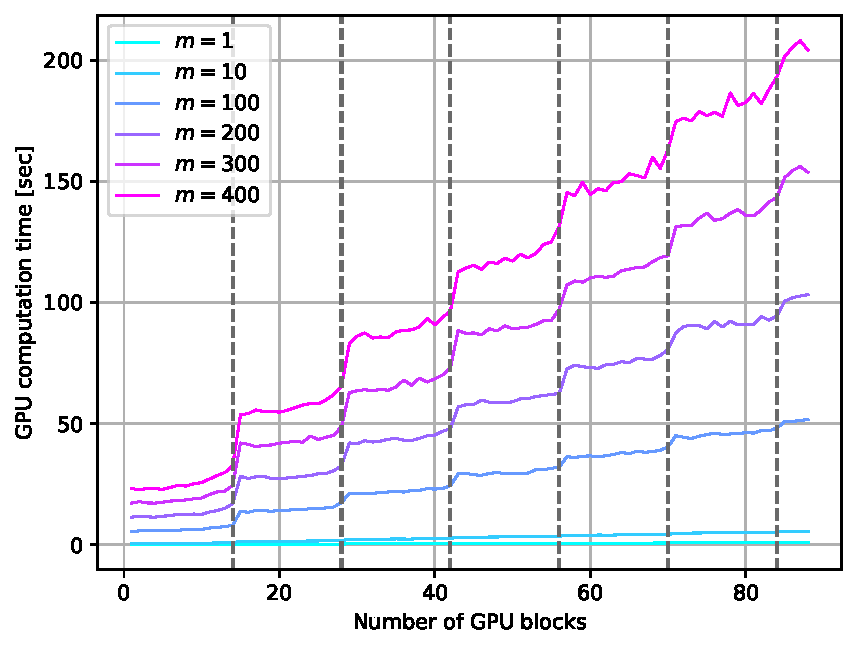
\includegraphics[scale=0.5]{graphs/ComputationTime_Tesla_GPUTimeVsNOfBlocks_VariousM_1000SimsPerThread.pdf}
    \caption{Tempi di esecuzione dell'algoritmo su GPU al crescere del numero di blocchi per diverse densità di date di rilevamento. Nelle simulazioni cronometrate in ogni blocco erano istanziati 512 \textit{thread}, ciascuno incaricato di eseguire 1000 simulazioni dell'evoluzione del prezzo del sottostante.}
    \label{fig:gpucomptime}
\end{figure}
\lipsum[1-3]

\subsection{(B-5-b) Analisi del fattore di guadagno GPU-CPU}
\lipsum[1-3]

\section{(B-6) Limiti di applicabilità e approssimazioni} \label{sec:limits}

\begin{figure}[t]
    \centering
    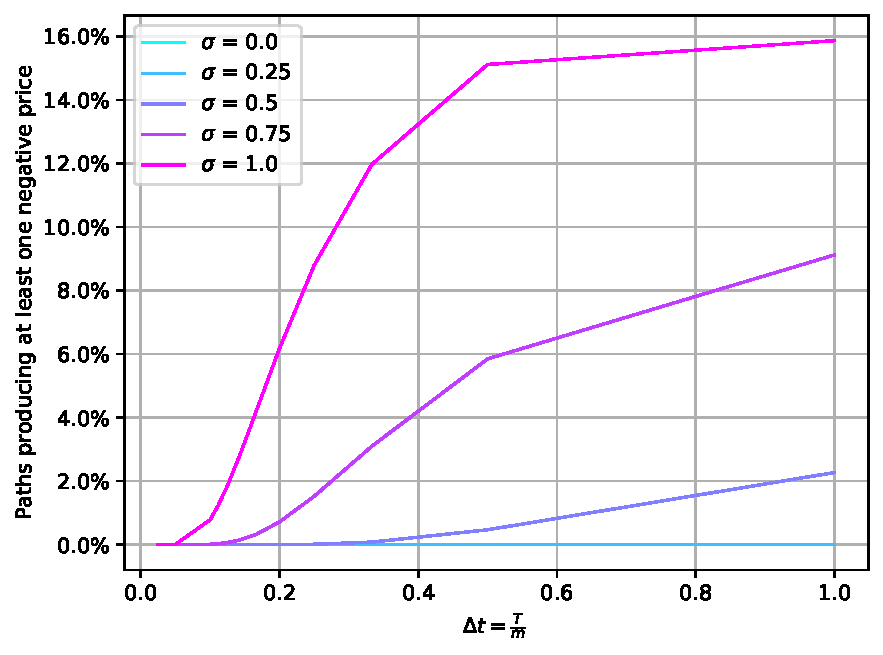
\includegraphics[scale=0.5]{graphs/NegativePrices_PercentageVsM_VariousSigmas.pdf}
    \caption{Percentuale di evoluzioni simulate del prezzo del sottostante che riportano almeno un'istanza di prezzo $S(t_i)$ negativo al variare della distanza temporale $\Delta t$ tra le date di rilevamento; curve di colore da \textit{ciano} a \textit{magenta} corrispondono a valori crescenti della volatilità $\sigma$ del mercato.}
    \label{fig:negativeprices}
\end{figure}
\lipsum[1-3]
\chapter{(C) Formule di valutazione esatte} \label{cap:exactformulas}

\section{(C-0) Formule analitiche per i limiti asintotici della barriera}
\lipsum[1-3]

\section{(C-1) Formula analitica per singola data di rilevazione}
\lipsum[1-3]

\section{(C-2) Formula analitica per date di rilevazione asintoticamente infinite}
\lipsum[1-3]
\chapter{(E) Processi stocastici} \label{cap:bimodal}

\section{(E-1) Sviluppo del processo lognormale a variabile stocastica binaria}

La determinazione del prezzo di un prodotto derivato è indissolubilmente legata all'andamento teorico del valore del sottostante. Data questa premessa, un equo \textit{pricing} delle opzioni non può prescindere da una previsione il più accurata possibile dell'andamento di tale valore. Nella Sezione \ref{sec:introduction_econophysic_option_pricing} è stato indicato lo schema del moto browniano geometrico come particolarmente valido per questo tipo di modellizzazione. Il processo lognormale con cui evolve il prezzo del sottostante è un processo di tipo markoviano descritto, come si è visto, dall'equazione a schema esatto \eqref{eq:exactprice}, dove $w$ rappresenta una variabile aleatoria a media nulla e varianza unitaria.

Nell'ottica di riprodurre con la maggiore fedeltà possibile un'ipotetica evoluzione dei prezzi del sottostante, il termine $w$ è stato estratto da una distribuzione gaussiana. Successivamente, a titolo di confronto, abbiamo implementato nella classe \codeword{RNG} e le sue derivate una nuova funzione \codeword{GetBimodal()} che genera una variabile stocastica dicotomica
\begin{equation}
    z = \begin{cases}
    +1, & \text{con probabilità} \,\, \frac{1}{2};\\
    -1, & \text{con probabilità} \,\, \frac{1}{2}.
  \end{cases}
    \label{eq:binary_variable}
\end{equation}
Abbiamo quindi applicato iterativamente il processo lognormale 
\begin{equation}
    S\left(t_{i+1}\right) = S(t_i) \exp{\left[\left(r - \frac{\sigma^2}{2}\right) \Delta t + \sigma \sqrt{\Delta t} z\right]}
    \label{eq:bimodal_price}
\end{equation}
con questa nuova variabile per valutare l'effetto che essa induce sulla stima del prezzo dell'opzione se raffrontata ai risultati conseguiti con una variabile gaussiana $w$.

Nel caso dicotomico, per ogni intervallo temporale $\Delta t$ il valore di $S(t_{i + 1})$ è vincolato a due sole possibilità rispetto a $S(t_i)$, ovvero quella di un movimento al rialzo, se $z = 1$, o al ribasso, se $z = -1$. A ogni passo della simulazione il prezzo $S(t)$ può quindi assumere due soli valori dipendenti dal risultato del passo precedente, dalla volatilità $\sigma$, dal tasso di interesse privo di rischio $r$ e dalla scelta dell'intervallo stesso $\Delta t$, in contrapposizione allo spettro continuo di valori del processo lognormale standard.

\section{(E-2) Convergenza del processo binario al processo lognormale gaussiano}

Sia che si scelga di utilizzare una variabile $w$ a distribuzione gaussiana, sia che il termine aleatorio sia di tipo bimodale $z$, la funzione \codeword{ExactLogNormalStep(...)}, che prende in ingresso la variabile stocastica e restituisce il prezzo del sottostante alla data di rilevazione considerata, è la medesima, in quanto l'equazione \eqref{eq:exactprice} si applica identicamente all'uno e all'altro caso. 

Abbiamo eseguito una serie di coppie di simulazioni identiche a eccezione del tipo di parametro pseudocasuale passato alle funzioni del processo lognormale. In questo modo è stato possibile confrontare i risultati relativi a entrambe le scelte del termine aleatorio per verificarne la convergenza.

In particolare, le simulazioni prese in esame per la comparazione stimano il prezzo di opzioni del tipo \textit{plain vanilla call} a partire dai seguenti dati di \textit{input}:
\begin{itemize}
    \item numero di simulazioni $N={10}^7$;
    \item numero di intervalli temporali $m$ variabile tra $1$ e $350$.
\end{itemize}
In Figura \ref{fig:bimodal} sono riportati i risultati ottenuti per mezzo del processo lognormale esatto nel caso di impiego di una variabile gaussiana (in grigio, tratteggiato) oppure di una bimodale (in magenta).

\begin{figure}[t]
    \centering
    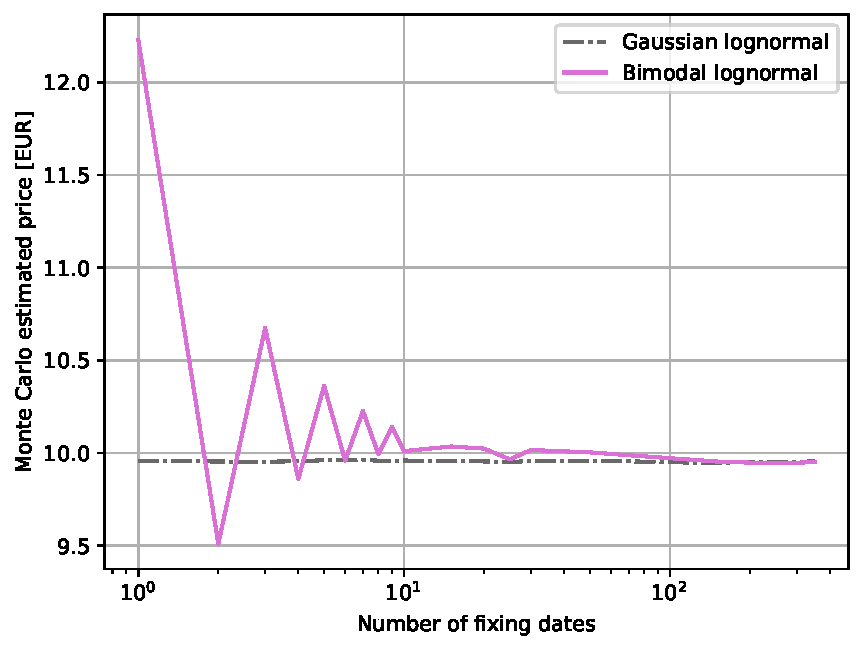
\includegraphics[scale=0.5]{graphs/OptionPriceBimodal_PriceVsM.pdf}
    \caption[Confronto tra il prezzo stimato dell'opzione \textit{performance corridor} sfruttando variabili  bimodali e gaussiane di media nulla e varianza unitaria.]{Prezzo stimato dell'opzione \textit{performance corridor} tramite lo schema lognormale esatto sfruttando variabili pseudocasuali bimodali (in \textit{magenta}) e gaussiane di media nulla e varianza unitaria (in \textit{grigio, tratteggiato}).}
    \label{fig:bimodal}
\end{figure}

L'evoluzione delle due curve incontra le nostre aspettative: si nota infatti come, dopo un'iniziale fase discordante, i due sviluppi tendano a sovrapporsi e in particolare sia l'andamento della curva a variabile bimodale a stabilizzarsi fino a convergere sui risultati di quella a variabile gaussiana.
%La spiegazione risiede nella natura \textit{markoviana} del processo di calcolo: lo schema lognormale si basa su una successione ricorsiva che estrapola il prezzo al tempo $t_i$ a partire da quello alla data precedente $t_{i-1}$. Di conseguenza, nel caso non ci siano <<tappe temporali intermedie>>, i prezzi al \textit{tempo di maturità} sono l'esito di un'unica operazione in positivo o negativo. I risultati ottenuti dal singolo \textit{thread} si raggruppano dunque in due classi di prezzi. Incrementando il numero di passaggi intermedi aumenta il ventaglio di prezzi ottenibili dalla singola simulazione. Per una densità di date di rilevazione sufficientemente elevata i due processi danno risultati confrontabili, sebbene l'impiego di una variabile dicotomica non permetta di parlare di tendenza asintotica; infatti, al crescere di $m$ il prezzo finale del metodo binario non si avvicina indefinitamente <<dall'alto>> o <<dal basso>> al valore gaussiano.
Una spiegazione matematica di questo comportamento è fornita dal \textit{teorema del limite centrale}, secondo il quale la somma di $N$ variabili aleatorie $x_n$ indipendenti e identicamente distribuite tende, per $N \rightarrow \infty$, a seguire una distribuzione normale di media $N\braket{x_n}$ e varianza $N\text{Var}[x_n]$.

Considerando ora l'equazione che descrive l'andamento del prezzo del sottostante in funzione di $\Delta t$ e del numero $m$ di sottointervalli temporali di rilevazione
\begin{equation}
    S(m \Delta t) = S(0) \exp{\left[m \left(r - \frac{\sigma^2}{2}\right) \Delta t + \sigma \sqrt{\Delta t} \displaystyle\sum_{i=1}^m z_i\right]},
    \label{eq:price(n)}
\end{equation}
si può pensare di definire una nuova variabile aleatoria
\begin{equation}
   Y(m) \coloneqq \displaystyle\sum_{i=1}^m z_i.
\end{equation}

Le variabili ${z_i}$, siano esse bimodali o gaussiane, sono  pseudocasuali, indipendenti ed estratte secondo la medesima distribuzione: essendo soddisfatte le ipotesi del teorema del limite centrale, $Y(m)$ è quindi a sua volta una variabile che segue una distribuzione normale con media
\begin{equation}
    \braket{Y(m)} = m\braket{z_i} = 0,
\end{equation}
e varianza
\begin{equation}
    \text{Var}[Y(m)] = m\text{Var}[z_i] = m.
\end{equation}

La ragione della convergenza risiede dunque nel fatto che le variabili gaussiane e bimodali sono estratte con medesima media nulla e varianza unitaria, il che, in virtù del teorema del limite centrale, porta $Y(m)$ a coincidere nei due casi per $m\gtrsim 100$; al di sotto di tale limite il teorema non è più valido e la natura dicotomica della variabile $z$ induce la dispersione osservabile rispetto al processo lognormale standard. L'andamento riscontrato nelle simulazioni ha quindi una comprova teorica.

\chapter{(F) Programmazione in CUDA di tipo avanzato} \label{cap:cudacpp}

\section{(F-1) Note sull'implementazione della struttura a classi nella libreria}
In ragione dell'elevata complessità dei risultati richiesti e delle tempistiche prolungate di sviluppo, la libreria di \textit{pricing} esposta in questa relazione è stata fin dal principio da noi concepita in un'ottica di massima estensibilità, incapsulando le funzioni chiave per i nostri scopi in classi C++ secondo il paradigma della programmazione orientata agli oggetti. Ciò emerge con estrema chiarezza nella classe \codeword{Data_stream_manager}, progettata per la gestione dei flussi di \textit{input} e \textit{output}: nonostante la libreria sia stata progressivamente ampliata con opzioni accessorie quali il confronto dei tempi di esecuzione in GPU e GPU oppure la scelta di una variabile stocastica gaussiana o binaria, la varietà di strutture dati ha permesso di non modificare mai la segnatura del metodo \codeword{ReadInputData(...)}, atto alla lettura dei dati in ingresso da un file \codeword{input.dat} in continuo mutamento.

Un discorso a parte va fatto per l'introduzione della variabile bimodale oggetto di studio del Capitolo \ref{cap:bimodal}. Non lavorando in un ambiente di programmazione procedurale, la nostra scelta per l'implementazione è stata di definire un nuovo metodo virtuale \codeword{GetBimodal()} all'interno della classe \codeword{RNG}: così facendo non è stata necessaria alcuna modifica della classe \codeword{Path}, in quanto il processo lognormale in schema esatto \eqref{eq:exactprice} si adattava già perfettamente ai nostri scopi. Per applicare questa strada abbiamo però dovuto modificare a cascata tutti i generatori concreti derivati da \codeword{RNG}, operazione che in ambito procedurale non sarebbe necessariamente fattibile.

A riprova dell'efficacia di un'architettura a classi, tuttavia, possiamo citare opzioni più dispendiose dal punto di vista della scrittura del codice ma del tutto applicabili in un paradigma a \textit{subroutine}. Un approccio ideale nelle prime fasi di progettazione del codice sarebbe stato separare la classe per la generazione di numeri pseudocasuali da quella che definisce le distribuzioni di estrazione, su modello dei generatori implementati nella libreria C++11 \codeword{<random>}. Combinando questo accorgimento con la scrittura di un nuovo metodo \codeword{BimodalStep(double)} nella classe \codeword{Path}, ciò avrebbe garantito estensibilità anche nel caso di processi diversi dai due lognormali già presenti senza apportare cambiamenti significativi alla funzione di \textit{pricing} principale.

Concludiamo menzionando un altro vantaggio del paradigma a classi da noi riscontrato, ovvero la possibilità di <<nascondere>> efficacemente i meccanismi interni della libreria all'utente. Un caso esemplare è fornito nuovamente dalla classe \codeword{RNG}: ogni generatore è dotato di un metodo \codeword{SetInternalState(RNG*)} che permette di inizializzarlo senza preoccuparsi del numero di \textit{seed} interni necessari a partire da un puntatore a un generatore qualunque. Nel contesto di programmazione su GPU, ciò ha altresì permesso di risparmiare spazio in memoria evitando di allocare una matrice di $4 N_\text{thread}$ \codeword{unsigned int} necessari per istanziare un generatore combinato indipendente per \textit{thread}. \cleardoublepage
% BACK MATTER
\setcounter{page}{0}
\pagenumbering{roman}
\appendix
\chapter{Listato commentato del codice} \label{app:allcode}
\lipsum[1-3]
%\addcontentsline{toc}{chapter}{Bibliografie}
%\begin{multicols}{2}
%\bibliographystyle{unsrt}
%\bibliography{Landslide_Literature.bib}
%\end{multicols}

%\cleartoleftpage{}
%

% ----------------------- Achterblad ------------------------------
% Vergeet niet de tekst aan te passen:
% - Afdeling
% - Adres van de afdeling
% - Telefoon en faxnummer
% -----------------------------------------------------------------
\thispagestyle{empty}
\sffamily
%
\begin{textblock}{191}(113,-11)
{\color{blueline}\rule{160pt}{5.5pt}}
\end{textblock}
%
\begin{textblock}{191}(168,-11)
{\color{blueline}\rule{5.5pt}{59pt}}
\end{textblock}
%
\begin{textblock}{183}(-24,-11)
\textblockcolour{}
\flushright
\fontsize{7}{7.5}\selectfont
\textbf{AFDELING}\\
Straat nr bus 0000\\
3000 LEUVEN, BELGI\"{E}\\
tel. + 32 16 00 00 00\\
fax + 32 16 00 00 00\\
www.kuleuven.be\\
\end{textblock}
%
\begin{textblock}{191}(154,-7)
\textblockcolour{}
\includegraphics*[height=16.5truemm]{Figuren/sedes}
\end{textblock}
%
\begin{textblock}{191}(-20,235)
{\color{bluetitle}\rule{544pt}{55pt}}
\end{textblock}





% ----------------------- Eigenlijke thesis -----------------------
% Vanaf de inleiding/het eerste hoofdstuk.
% -----------------------------------------------------------------
%\setcounter{page}{0}
%\pagenumbering{arabic}


\newpage



\end{document}
